\documentclass[border=10pt,tikz]{standalone}
\usepackage{tikz}
\usepackage{tikz-timing}
\usepackage{fontspec}
\setmainfont{Apple SD Gothic Neo}
\setsansfont{Apple SD Gothic Neo}
\usetikztiminglibrary{counters,interval,nicetabs}
\begin{document}
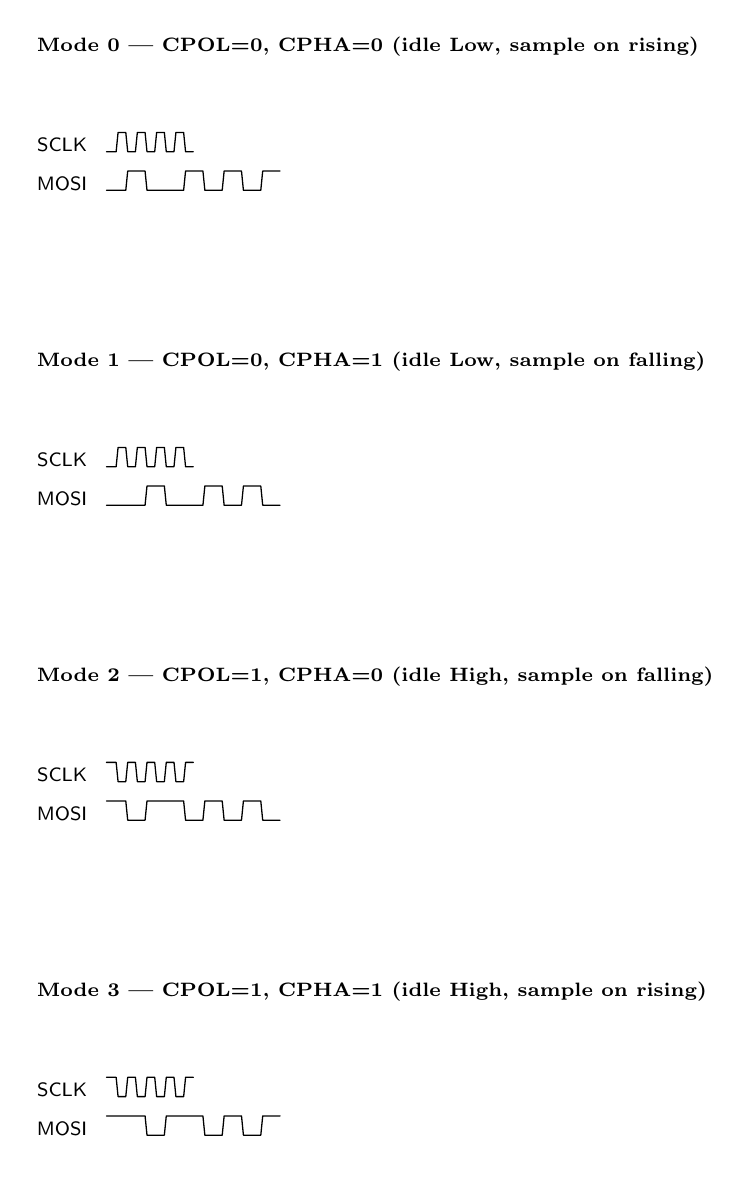
\begin{tikzpicture}[font=\scriptsize]

% Mode 0
\node[font=\scriptsize\bfseries, anchor=west] at (0, 8) {Mode 0 — CPOL=0, CPHA=0 (idle Low, sample on rising)};
\node[anchor=west] at (0, 6.5) {\begin{tikztimingtable}[xscale=1.4, yscale=1.4]
  SCLK & lhlhlhlhl \\
  MOSI & L H L L H L H L H \\
\end{tikztimingtable}};

% Mode 1
\node[font=\scriptsize\bfseries, anchor=west] at (0, 4) {Mode 1 — CPOL=0, CPHA=1 (idle Low, sample on falling)};
\node[anchor=west] at (0, 2.5) {\begin{tikztimingtable}[xscale=1.4, yscale=1.4]
  SCLK & lhlhlhlhl \\
  MOSI & L L H L L H L H L \\
\end{tikztimingtable}};

% Mode 2
\node[font=\scriptsize\bfseries, anchor=west] at (0, 0) {Mode 2 — CPOL=1, CPHA=0 (idle High, sample on falling)};
\node[anchor=west] at (0, -1.5) {\begin{tikztimingtable}[xscale=1.4, yscale=1.4]
  SCLK & hlhlhlhlh \\
  MOSI & H L H H L H L H L \\
\end{tikztimingtable}};

% Mode 3
\node[font=\scriptsize\bfseries, anchor=west] at (0, -4) {Mode 3 — CPOL=1, CPHA=1 (idle High, sample on rising)};
\node[anchor=west] at (0, -5.5) {\begin{tikztimingtable}[xscale=1.4, yscale=1.4]
  SCLK & hlhlhlhlh \\
  MOSI & H H L H H L H L H \\
\end{tikztimingtable}};

\end{tikzpicture}
\end{document}
